\section{Wide and Deep Neural Extractive Model}
\label{sec:model}
In this section, we describe our extractive model for product short title extraction. 
The overall architecture of our neural network based extractive model is shown in \figref{fig:overview}.
Basically, we use a Recurrent Neural Network (RNN) as the main building block of the sequential classifier. 
However, unlike traditional RNN-based sequence labeling models used in NER or 
POS tagging, where all the word level features are fed into RNN cell, 
we instead divide the features into three parts, 
namely \emph{Content}, \emph{Attention} and \emph{Semantic} respectively. 
Finally we combine all three features in an ensemble.

\begin{figure*}[h]
	\centering
	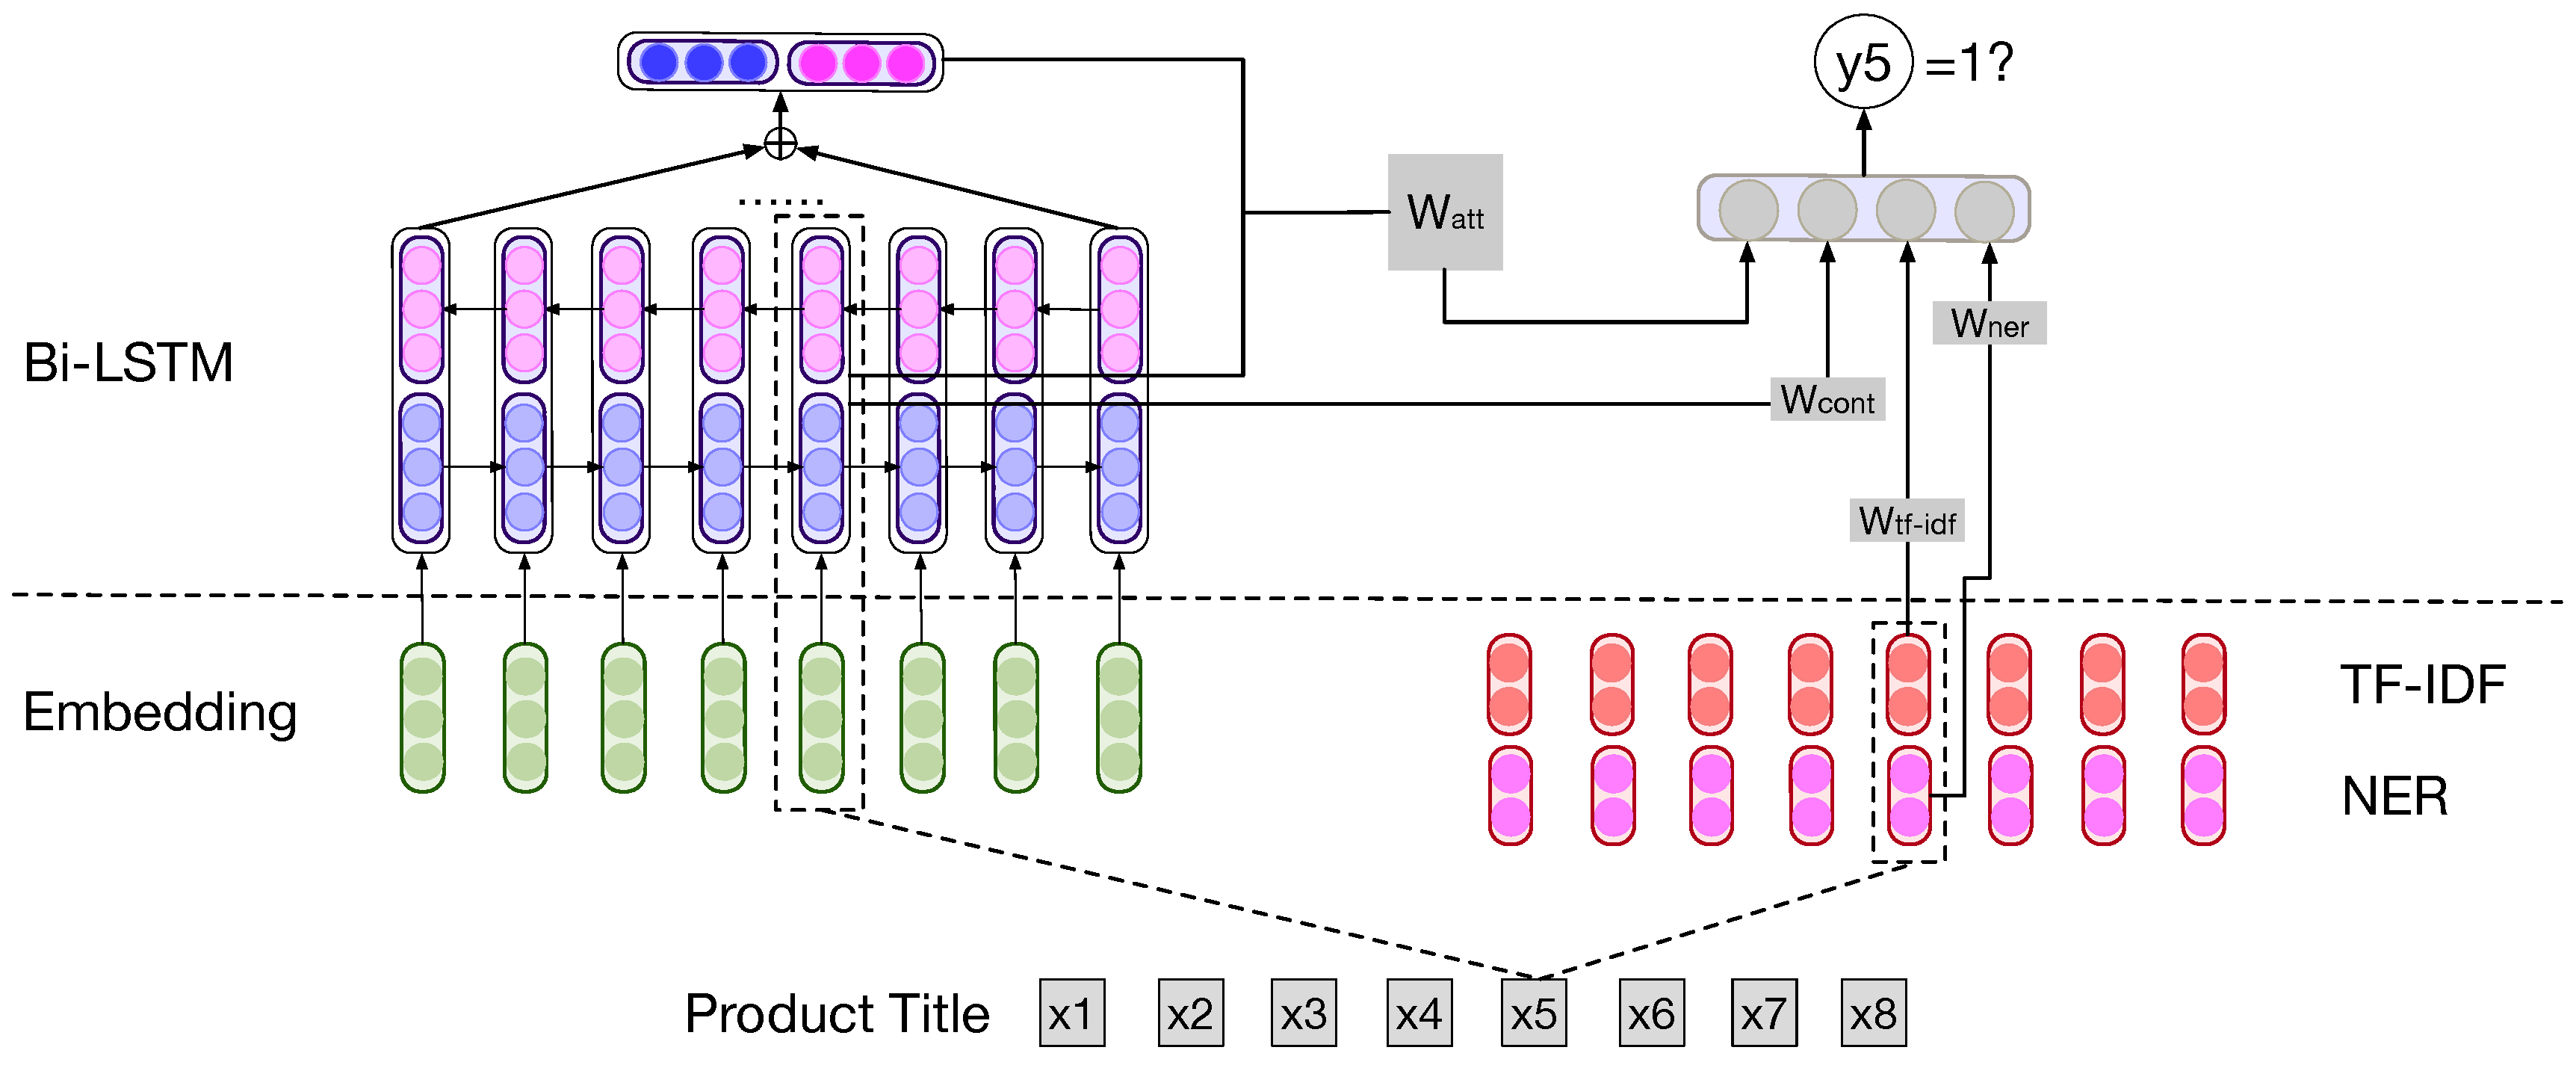
\epsfig{file=fig/overview.eps, angle=0, width=2.0\columnwidth}
	\caption{Architecture of Wide and Deep Neural Extractive Model.}
	\label{fig:overview}
%	\vspace{-10pt}
\end{figure*}

\subsection{Content Feature}
RNNs are a powerful family of neural networks designed for sequential data and 
have shown great promise in many NLP tasks. RNNs take a sequence of 
vector $(\bi{x}_1, \bi{x}_2, \dots, \bi{x}_n)$ and return another sequence 
$(\bi{h}_1, \bi{h}_2, \dots, \bi{h}_n)$ that represents the hidden state information 
about the sequence at each time step in the input. In theory, 
RNNs can learn long dependencies but in practice they seem to be biased towards 
their most recent inputs of the sequence. Thus, LSTMs \cite{hochreiter1997long} 
are proposed and they have shown greater capabilities to 
capture long-range dependencies.

To encode the product title, we first look up an embedding matrix $E_x\in \textbf{R}^{d\times v}$ to get the word embeddings $\bi{X}=(\bi{x}_1, \bi{x}_2, \dots, \bi{x}_n)$. 
Here, $d$ denotes the dimension of the embeddings and $v$ denotes the vocabulary size of natural language words. 

If we use unidirectional LSTM, the outcome of current word is only based on the words before it so the information of the words after it is totally lost. 
To avoid this, we use bi-LSTM which consists of a forward network that handles 
the sequence from left to right and a backward network that does the reverse.
Then, the embeddings are fed into a bidirectional LSTM networks.
To this end, we get two hidden state sequences, $(\overrightarrow{\bi{h}_1}, \overrightarrow{\bi{h}_2}, \dots, \overrightarrow{\bi{h}_n})$ from the forward network and $(\overleftarrow{\bi{h}_1}, \overleftarrow{\bi{h}_2}, \dots, \overleftarrow{\bi{h}_n})$ from the
backward network. 
We concatenate the forward hidden state of each word with corresponding backward hidden state, 
resulting in a representation $[\overrightarrow{\bi{h}_i};\overleftarrow{\bi{h}_i}]$. 
At this point, we obtain the representation of the product title $X$.

The \textit{content} feature of current word $x_i$ is then calculated as:
\begin{equation}
\label{eqn:content}
\bi{f}_{cont} = \bi{W}_{cont}^T [\overrightarrow{\bi{h}_i};\overleftarrow{\bi{h}_i}] + \bi{b}_{cont},
\end{equation}
where $\bi{W}_{cont}$ and $\bi{b}_{cont}$ are model parameters.

%We adopt bi-directional long short-term memory (Bi-LSTM) as our RNN implementation,
%and it can be considered as a word level feature representation.

%LSTM introduces gate mechanism and memory cell to maintain long dependency information
%and avoid gradient vanishing.

%In order to incorporate information
%from both sides of sequence, we use bi-directional
%LSTM (Bi-LSTM) with forward and backward directions.

\subsection{Attention Feature}

Attention mechanisms \cite{bahdanau2014neural,luong2015effective} have become an integral part of sequence modeling and transduction models in various NLP tasks, which allows better understanding of sequential data.
In order to measure the importance of each word relevant to the whole product title, we borrow the idea of attention mechanism \cite{bahdanau2014neural,luong2015effective} to calculate a relevance score between the hidden vector of current word and representation of the entire title sequence.

The representation of the entire product title is modeled as a non-linear transformation of the average pooling of the concatenated hidden states of the BiLSTM:

\begin{equation}
\bi{d}=\tanh{(\bi{W}_d{\frac{1}{n}}\sum_{j=1}^{n}{[\overrightarrow{\bi{h}_i};\overleftarrow{\bi{h}_i}]}+\bi{b}_d)}.
\end{equation}

Therefore, the attention feature of current word $x_i$ is calculated by a Bilinear combination function as:
\begin{equation}
\label{eqn:attention}
\bi{f}_{att} = \bi{d}^T\bi{W}_{att} [\overrightarrow{\bi{h}_i};\overleftarrow{\bi{h}_i}] + \bi{b}_{att},
\end{equation}
where $\bi{W}_{att}$ is a parameter matrix.

\subsection{Semantic Feature}

Apart from the two hidden features calculated using an RNN encoder, 
we design another kind of feature including TF-IDF and NER Tag, 
to capture the deep semantics of each word in a product title.

\subsubsection{TF-IDF}

Tf-idf, short for term frequency–inverse document frequency, 
is a numerical statistic that is intended to reflect how important a word is to a document in corpus or a sentence in a document.

A simple choice to calculate term frequency of current word $x_i$ is to use the 
number of its occurrences (or count) in the title:

\begin{equation}
\label{eqn:tf}
\textbf{tf}(x_i, X) =\frac{cnt_{x_i}}{n}.
\end{equation}

In the case of inverse document frequency, we calculate it as:

\begin{equation}
\label{eqn:idf}
\textbf{idf}(x_i) =\log(1+\frac{N}{C_{x_i}}),
\end{equation}
where $N$ is the number of product titles in the corpus and $C_{x_i}$ is the number of titles containing the word $x_i$.

By combining the above two, the tf-idf score of word $x_i$ in a product title $X$, denoted as $\textbf{tf-idf}(x_i, X)$, is then calculated as the product of $\textbf{tf}(x_i, X)$ and $\textbf{idf}(x_i)$.

We design a feature vector containing three values: tf score, idf score and tf-idf score and the calculate a third feature:

\begin{equation}
\label{eqn:tf-idf}
\bi{v}_{tfidf} = [\textbf{tf}(x_i, X); \textbf{idf}(x_i); \textbf{tf-idf}(x_i, X)]
\end{equation}

\begin{equation}
\bi{f}_{tfidf} =\bi{W}_{tfidf}^T \bi{v}_{tfidf} + \bi{b}_{tfidf}.
\end{equation}


\subsubsection{NER}   

Named Entity Recognition (NER) is a fundamental NLP task, which aims to identify
named entities such as PERSON, LOCATION and ORGANIZATION in natural language text.
We use a specialized NER tool for E-commerce to label entities in 
a product title. In total there are $36$ types of entities, which are of 
common interest in E-commerce scenario, such as ``颜色''(color), 
``风格''(style) and ``尺寸规格 ''(size).
For example, in segmented product title ``包邮 Nike 品牌 的 红色 运动裤'' 
(Nike red sweatpants with free shipping),
``包邮 ''(Free shipping) is labeled as \emph{Marketing\_Service},
``Nike'' is labeled as \emph{Brand}, ``红色''(Red) is labeled as \emph{Color}
and ``运动裤''(Sweatpants) is labeled as \emph{Category}.
We use one-hot representation to encode NER feature $\bi{v}_{ner}$ of each word and 
then integrate it into the model by proposing a fourth feature:

\begin{equation}
\label{eqn:ner}
\bi{f}_{ner} = \bi{W}_{ner}^T \bi{v}_{ner} + \bi{b}_{ner}.
\end{equation}

\subsection{Ensemble}
\label{sec:inference}
We combine all the features above into one final score of word $x_i$:

\begin{equation}
\label{eqn:ner}
score_i = \sigma(\bi{W}_{f}^T [\bi{f}_{cont};\bi{f}_{att};\bi{f}_{tfidf};\bi{f}_{ner}] + \bi{b}_{f}),
\end{equation}
where $\sigma$ is the sigmoid or logistic function, which restrain the score between $0$ and $1$. Based on that, we set a threshold $\tau$ to decide whether we keep word $x_i$ in the short title or not.

Our model is very much like the Wide \& Deep Model architecture \cite{cheng2016wide}.
While the \textit{content} and \textit{attention}  features are deep since they rely on deep RNN structure, the \textit{semantic} features are relatively wide and linear.



%\subsection{Char-limit Constrained Inference}
%\label{sec:infer}
%
%\xusheng{Move this subsection to Discussion}
%As mentioned in \secref{sec:problem}, the word number of the short title can be strictly limited to a fixed number $m$ in some restrictive cases, due to the limited display space on mobile phones or other devices.
%
%This problem is similar as classic Knapsack Problem, where each term $x_i$ in the product title is an item with weight $len(x_i)$ and value $score_i$,
%where $len(x_i)$ represents the word (char) length of term $x_i$
%and $score_i$ represents the predicted likelihood of term by the model.
%The maximum weight capacity of our knapsack is $m$. 
%Then the target is:
%$$
%max \sum_{i=1}^{n} score_i z_i 
%$$
%$$
%s.t. \sum_{i=1}^{n} len(x_i)z_i \le m, z_i \in \{0, 1\}
%$$
%Where $z_i=1$ means $x_i$ should be resevered in the short title.
%
%Similar as solving 0-1 Knapsack Problem, we use an algorithm shown in \algoref{alg:inference}, with the idea of Dynamic Programming. 
%
%\begin{algorithm}
%	\small
%	\caption{Char-limit Constrained Inference}
%	\label{alg:inference}
%	\textbf{Input}: Sequence of term length $l$, Sequence of term score $s$, Limited char number $m$.
%	
%	\textbf{Output}: Sequence of 0-1 indicator $z$.
%	\begin{algorithmic}[1]
%		\Procedure{Predict}{$l, s, m$}
%		\State $z \gets 0$
%		\State $F \gets 0$
%		\For {$i$ = $1$ to $n$} 
%		\For {$j$ = $l_i$ to $m$}
%		\If {$F(i, j-l_i)+s_i > F(i, j)$}
%		\State $F(i, j) \gets F(i, j-l_i)+s_i$ 
%		\EndIf
%		\EndFor
%		\EndFor
%		
%		\For {$i$ = $n$ to $1$} 
%		\If {$F(i, m) = F(i-1, m)$}
%		\State $z_i \gets 0$
%		\Else 
%		\State $z_i \gets 1$
%		\State $m \gets m-l_i$
%		\EndIf
%		\EndFor
%		
%		\State \Return {$z$}
%		
%		\EndProcedure
%	\end{algorithmic}
%\end{algorithm}

